\documentclass{article}
\title{Neural Codec Language Models are
Zero-Shot Text-to-Speech Synthesizer (Summary)}
\author{Wang, et al. Microsoft (2023)}
\setlength{\parindent}{0pt}
\usepackage{enumitem}
\setlist[itemize]{label=\alph*., leftmargin=*}
\setlist[enumerate]{label=\arabic*., leftmargin=*}
\usepackage{graphicx} 

\begin{document}
\maketitle
\textbf{Index Terms:} VALL-E, TTS, Transformer, semi-supervised learning


\section{Highlight of this paper}
1. Zero-shot: only need an acoustic prompt for 3 seconds with its large and diverse dataset (60k+ hours)

2. pipeline: phoneme -$>$ discrete code -$>$ waveform

3. in-context learning ability in inference

4. keep the acoustic environments and speakers' emotions. 

\vspace{-10pt}
\section{Their work}
\vspace{-5pt}
1. demo page: https://aka.ms/valle

2.  follows the line of cascaded TTS but first uses audio codec code as intermediate representations. It is the first one that has strong in-context learning capabilities as GPT-3, which does not require fine-tuning, pre-designed features, or a complex speaker encoder

\vspace{-10pt}
\section{Implement Steps}
\vspace{-5pt}
3 stages in all. 

\vspace{-10pt}
\subsection{Terminology and Background Information}

\textbf{Embedding:} vectorise every word into a vector, and can tell the relationship between them by calculating the cosine-similarity. 

$\vec{E}(father)-\vec{E}(mother) \approx \vec E (male)-\vec E(female)$

\subsection{Speech Quantization}
Now, we have a dataset $D = \{x_i, y_i\}$ with $x_i$ are .wav files and $y_i$ are .txt files (labels).

First, we should transform each waveform file $x_i$ into an acoustic matrix $C$, i.e., Quantized Tokens. 

Formally, the waveform is 24kHz, but it is too large for prompt. We could sample it into 75 Hz. A 10-second audio should have $75\times 10=750$ frames. 

\vspace{5pt}
Secondly, to transform labels into phonemes, we use another off-the-shelf package `G2P`. 

\subsection{Training}

\begin{figure}[h]
    \centering
    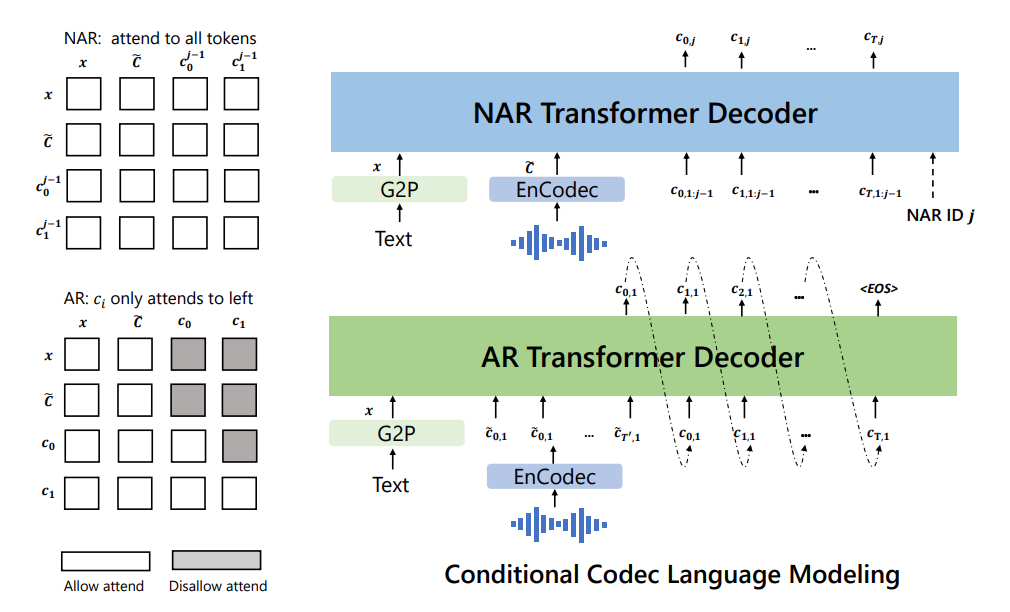
\includegraphics[width=0.9\linewidth]{training.png}
    \caption{Training}
    
\end{figure}

For each data in the dataset, we denote $C$ as the acoustic matrix and $x$ as the phoneme prompt. We denote the front few frames of $C$ as $\tilde C$. 


\subsubsection{AR model}
As shown in Figure 1, the 1st layer would be trained by the AR model. The data of the current frame is only allowed to be contributed by the\textbf{ last frame}. It is trained like a string of beans. 


GPT-3 has a similar principle, which maximizes the possibility of the next word, while VALL-E predicts the next frame. 

\vspace{5pt}
To express in a formula, 
\vspace{-15pt}
\[
maximize_{\theta_{AR}}\ p(C_{:,1}|x, \tilde{C}_{:,1};\theta_{AR})=\prod_{t=0}^T p(C_{t,1}|C_{<t,1},\tilde{C}_{:,1}, x;\theta_{AR})
\]

\subsubsection{NAR model}
In the following layers between 2 to 8, we use NAR model with its better performance in speed. That's because NAR could update in parallel. 

In this model, \textbf{all the frames in front of} $t$ could contribute to the frame of $t$. 

The formula should be the same. But the model inside is different. 

\subsection{Inference}
It has a similar process of training while using the input $\tilde C$ and $x$. However, it wouldn't need to feedback anything to the model. 

Usually, we would take $\tilde C$ as the prompt. In other words, we generate what we want directly after the audio we provide. So, intuitively, if the sentence is semantically continuous, the quality of output would be better. 

\section{Explanation}

\subsection{speech quantization}
\begin{figure}[h]
    \centering
    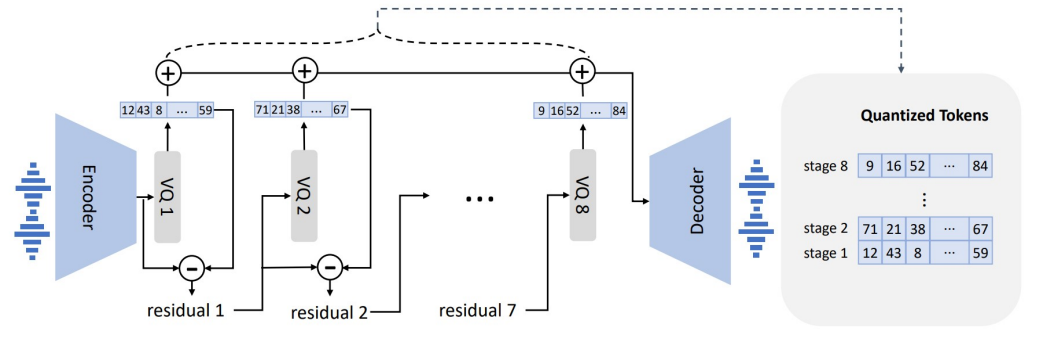
\includegraphics[width=1\linewidth]{Speech Quantization.png}
    \caption{Speech Quantization}
\end{figure}

We have 8 quantizers. The first one is to recover acoustic properties like speaker identity, while the following one learn more details. The first one plays the most important role. 

Geometrically, we could imagine a speech space with 8 dimensions. Take the first VQ as an example, we can recognise the waveform as a vector in the space. `residual 1` is just the difference between the centre of 1st dim and the real audio. We plug the residual 1 into VQ 2 and conduct the same operation, and finally, we can decompose the waveform into the matrix. 
\subsection{training}

The training process could be divided into two parts: forward and backward. 

We use the forward part to simulate the process of inference, from which we can derive loss (the difference between target and output, we would use Cross Entropy Loss). 

After that, we will conduct a backward process to modify the parameter $\theta$ to narrow the loss. 

Here, the acoustic matrix for the dataset is $C^{T\times 8}$, and the parameter $\theta$ is an abstract parameter and has already been embedded into the model. In the aspect of coding, we chose the model named \textbf{Llama}. 

\subsubsection{Why do we choose different models for different layers? }
It's a trade-off between quality and speed. 

On the one hand, AR model is good at adapting to the different speaking speeds of the enrolled recordings. 

On the other hand, compared with AR model, NAR model runs way faster than AR since it could better parameters more freely. It reduces the Time Complexity from $O(T)$ to $O(1)$


\vspace{5pt}
\textbf{The purpose of all the training is to better the parameter $\theta$ and decrease the loss. } 

\end{document}

